\documentclass[border=10pt]{standalone}
\usepackage{pgfplots}
\pgfplotsset{compat=1.18, trig format plots=rad}
\begin{document}
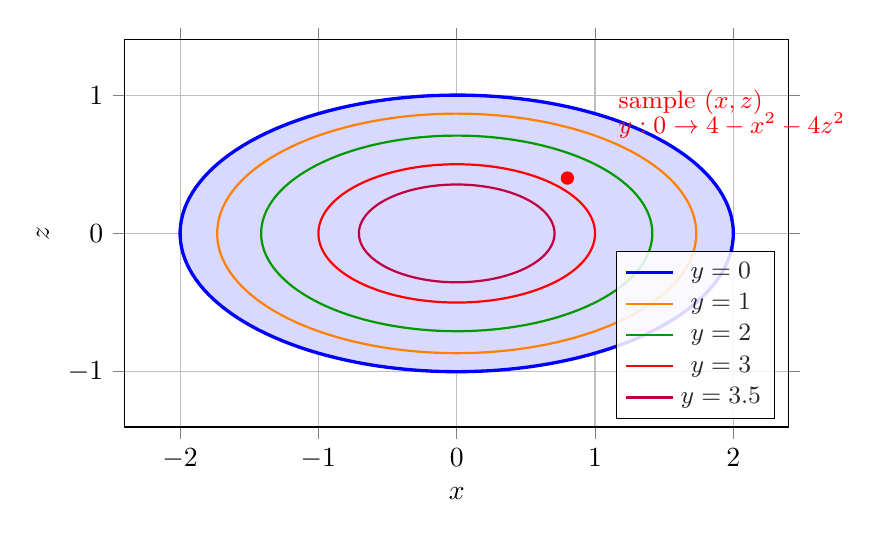
\begin{tikzpicture}
\begin{axis}[
    axis equal image,
    xmin=-2.4, xmax=2.4, ymin=-1.4, ymax=1.4,
    xlabel=$x$, ylabel=$z$,
    width=11cm, height=6.5cm,
    grid=both,
    tick align=outside,
    clip=false,
    legend style={at={(0.98,0.02)}, anchor=south east, font=\small, fill=white, fill opacity=0.85},
]
% filled projection D
\addplot[fill=blue!15, draw=none, domain=0:2*pi, samples=160, forget plot]
    ({2*cos(x)},{sin(x)}) \closedcycle;
% outer boundary y=0
\addplot[blue, very thick, domain=0:2*pi, samples=160] ({2*cos(x)},{sin(x)});
\addlegendentry{$y=0$}
% inner level curves
\addplot[orange, thick, domain=0:2*pi, samples=160] ({sqrt(3)*cos(x)},{sqrt(3)/2*sin(x)});
\addlegendentry{$y=1$}
\addplot[green!60!black, thick, domain=0:2*pi, samples=160] ({sqrt(2)*cos(x)},{sqrt(2)/2*sin(x)});
\addlegendentry{$y=2$}
\addplot[red, thick, domain=0:2*pi, samples=160] ({cos(x)},{0.5*sin(x)});
\addlegendentry{$y=3$}
\addplot[purple, thick, domain=0:2*pi, samples=160] ({sqrt(0.5)*cos(x)},{sqrt(0.5)/2*sin(x)});
\addlegendentry{$y=3.5$}
% sample point
\addplot[only marks, mark=*, red, mark size=2.2pt, forget plot] coordinates {(0.8,0.4)};
\node[red, anchor=west, font=\small] at (axis cs:1.1,0.95) {sample $(x,z)$};
\node[red, anchor=west, font=\small] at (axis cs:1.1,0.78) {$y:0\to 4-x^2-4z^2$};
\end{axis}
\end{tikzpicture}
\end{document}
